
\chapter{Projektion in OpenGL}

Durch die Objekterkennung und anschliessender Bestimmung von dessen Lage wurde ein wichtiger Teil zur Fertigstellung einer Augmented Reality Szene bereits erreicht. Im letzten Schritt geht es nun darum die Resultate aus den vorhergehenden Schritten zu verwenden und schlussendlich ein 3D-Objekt mit korrekter Perspektive in die Szene zu rendern.


\section{Livebild mittels Texturemapping}

Da wir für eine Augmented Reality Szene immer auch die Realität als Hintergrund betrachten wollen, müssen wir das Livebild der Kamera ebenfalls in die dreidimensionale Szene integrieren. Dies erreichen wir, indem wir für jedes Einzelbild der Kamera ein \textit{Texture Mapping} durchführen.
Der Ablauf des Texture Mappings kann vereinfacht mit folgenden Schritten in OpenGL aufgezeigt werden:

\begin{enumerate}
\item Das Bild wird in eine Textur konvertiert und auf die Grafikkarte hochgeladen.
\item Zeichne ein planares, rechteckiges Objekt in die Szene.
\item Entsprechend der definierten Textur-Koordinaten zeichnet die Grafikkarte die Oberfläche des Objekts mit der Textur.
\end{enumerate}

Ausserdem wird für diesen Schritt eine orthogonale Projektion durchgeführt, damit das gerenderte Hintergrundbild die gleichen Dimensionen hat, egal ob es sich im Vordergrund oder Hintergrund der Szene befindet. Wir können dadurch das Hintergrundbild weit nach hinten schieben, so dass es keine Kollision mit den später zu rendernden Objekten gibt.


\section{Transformation der extrinsischen Matrix}

Durch die Pose Estimation konnte bereits die extrinsische Matrix bestimmt werden. Damit ein in OpenGL gerendertes Objekt an derselben Position mit derselben Rotation wie das real erkannte Objekt erscheint, muss die extrinsische Matrix an OpenGL übergeben werden.


\begin{figure}[!ht]
\centering
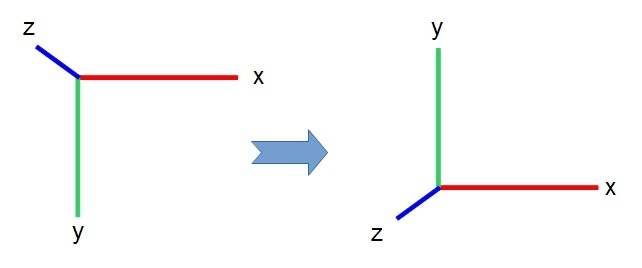
\includegraphics[scale=0.5]{images/opencv-to-opengl.jpg} 
\caption{Transformierung des Koordinatensystem von OpenCV (links) nach OpenGL (rechts).}
\label{fig:opencv-to-opengl}
\end{figure}


Die Matrix aus OpenCV kann jedoch nicht direkt an OpenGL übergeben werden, da beide unterschiedliche Koordinatensysteme verwenden. Die Abbildung \ref{fig:opencv-to-opengl} stellt diese Gegebenheit grafisch dar. Die Konvertierung kann mit einer einfachen Matrixmultiplikation erreicht werden, indem die Y- und Z-Achsen invertiert werden:

\begin{equation}
M_{OpenGL}
=
\begin{bmatrix}
1 & 0 & 0 & 0 \\
0 & -1 & 0 & 0 \\
0 & 0 & -1 & 0 \\
0 & 0 & 0 & 1
\end{bmatrix} 
[R | t]
\end{equation}

 
\section{Perspektivische Projektion}

Damit ein virtuelles Objekt sich in die reale Szene einfügen kann, muss die korrekte perspektivische Projektion gesetzt werden, nämlich dieselbe, welche auch die Kamera hatte, die das reale Bild aufgenommen hat. Die dazu benötigte Projektionsmatrix kann anhand der \textit{intrinsischen Parameter} abgeleitet werden. Ein Vergleich einer inkorrekten Projektionsmatrix mit einer korrekten ist in Abb. \ref{fig:opengl-perspektive} zu sehen.


\begin{figure}[!ht]
\centering
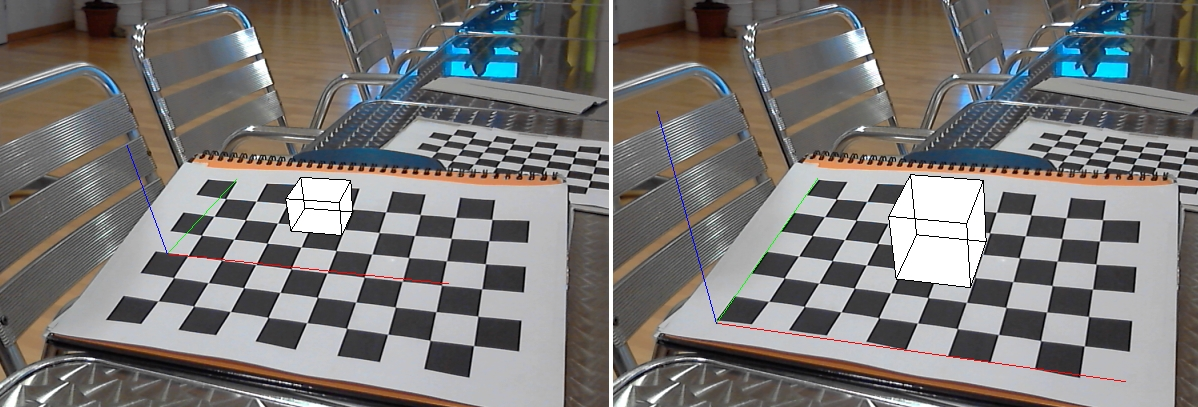
\includegraphics[scale=0.5]{images/opengl-perspective.jpg} 
\caption{Eine inkorrekt gesetzte perspektivische Projektion oder falsche intrinsische Parameter können das projizierte Objekt stark verfälschen.}
\label{fig:opengl-perspektive}
\end{figure}


K. Simek \cite{simek} erklärt die notwendigen Schritte, wie die perspektivische Projektion anhand der Kameramatrix gesetzt werden kann. Er teilt die Projektionsmatrix dazu in die Teile Perspektive und NDC (Normalized Device Coordinates) auf (Gleichung \ref{eq:projektion}).

\begin{equation}
Proj = NDC \times Persp
\label{eq:projektion}
\end{equation}

Der NDC kann in OpenGL mit einer orthogonalen Projektion umgesetzt werden. Die Perspektivenmatrix muss mit den kameraspezifischen intrinsischen Parametern ergänzt werden. $\alpha$ und $\beta$ entsprechen dabei der horizontalen und vertikalen Brennweiten der Kamera, $x_0$ und $y_0$ der Abweichung der optischen Bildmitte zum realen Bildzentrum. Die resultierende Projektionsmatrix kann später direkt in OpenGL angewandt werden.

\begin{equation}
Persp
=
\begin{bmatrix}
\alpha & 0 & -x_0 & 0 \\
0 & \beta & -y_0 & 0 \\
0 & 0 & near + far & near * far \\
0 & 0 & -1 & 0
\end{bmatrix} 
\end{equation}


\section{Positionierung der 3D Objekte}

Wie bereits in Kapitel \ref{sec:projektion-door} beschrieben, wurden die Objektpunkte einer Türe so definiert, dass die untere linke Ecke als Ursprungspunkt (0, 0) dient. Da es ein Ziel dieser Arbeit ist, ein Vordach über die Türe zu prjizieren, muss eine entsprechende Translation vorgenommen werden.

Da keine Kenntnisse über die realen Einheiten (siehe Kapitel \ref{sec:definition-objektpunkte}) bekannt sind, müssen wir die Translation entsprechend der Einheit der definierten Objektpunkte durchführen. Da die Breite der Türe als Einheitsgrösse 1 definiert wurde und die Höhe dem Verhältnis Höhe zu Breite entspricht, können wir die Model-View-Matrix um die halbe Breite (0.5) und die Höhe (r = Verhältnis Höhe zu Breite) verschieben (Abbildung \ref{fig:opengl-translation}).

\begin{equation}
M_{translation}
=
\begin{bmatrix}
1 & 0 & 0 & w/2 \\
0 & 1 & 0 & h \\
0 & 0 & 1 & 0 \\
0 & 0 & 0 & 1
\end{bmatrix} 
\end{equation}


\begin{figure}[!ht]
\centering
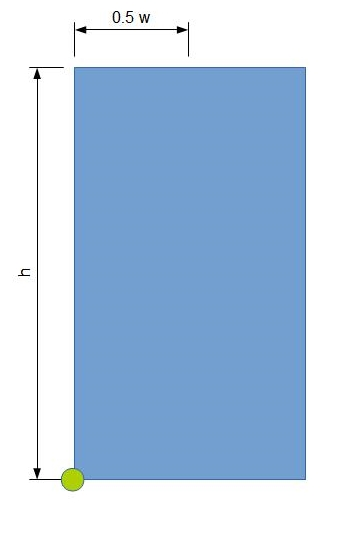
\includegraphics[scale=0.75]{images/opengl-translation.jpg} 
\caption{Schematische Darstellung der Translation von der unteren linken Ecke der Türe zur Oberkante.}
\label{fig:opengl-perspektive}
\end{figure}


\section{Konvertierung nach Core Profile}

Nach einer ersten funktionierenden Version der Schachbretterkennung inklusive Projektion und 3D-Rendering haben wir Zeit in die Konvertierung nach Core Profile OpenGL investiert. Diesen Schritt haben wir gewählt, weil die in dieser Version zur Verfügung stehenden Routinen ebenfalls auf den mobilen Versionen von OpenGL (OpenGL ES) zu finden sind und eine zukünftige Portierung dadurch erheblich vereinfacht wird. Core Profile wird aktuell auch als moderne Art der OpenGL-Entwicklung betrachtet und bietet eine vereinfachte API und bessere Performance.